\documentclass[a4paper,11pt]{article}
\usepackage{CAR}
\usepackage[T1]{fontenc}
\usepackage{amsfonts}
\usepackage{amsmath}
\usepackage{amssymb}
\usepackage{todo}

\begin{document}
\setcounter{footnote}{0}
\setcounter{figure}{0}


%%%%%%%%%%%%%%%%%%%%%%%%%%%%%%%%%%%%%%%%%%%%%%%%%%%%%%%%%%%%%%%%%%%%%%%%%%%%%%%%
% FOR THE AUTHORS
%%%%%%%%%%%%%%%%%%%%%%%%%%%%%%%%%%%%%%%%%%%%%%%%%%%%%%%%%%%%%%%%%%%%%%%%%%%%%%%%

\Aufsatz 
% Title
{Towards Post-Quantum Secure Symmetric Cryptography: \\
A Mathematical Perspective}
% Short title for the table of contents
{Towards Post-Quantum Secure Symmetric Cryptography}
% Authors
{X. Bogomolec, J. G. Underhill, S. A. Kovac}
% Label of authors' names
{NameAuthor}
% Names and adresses
{ Xenia Bogomolec, Quant-X Security {\&} Coding, Hanover\\ John Gregory Underhill, itk AVtobvS SARL, Fribourg\\  Stiepan Aurélien Kovac, QRCrypto SA, Fribourg \\}
% Images of authors
{./ITK.jpg}
% E-Mails
{xb@quant-x-sec.com,john.underhill@protonmail.com,contact@qrcrypto.ch,}



%%%%%%%%%%%%%%%%%%%%%%%%%%%%%%%%%%%%%%%%%%%%%%%%%%%%%%%%%%%%%%%%%%%%%%%%%%%%%%%%
% IF THE ARTICLE IS WRITTEN IN ENGLISH, THEN UNCOMMENT
% THE NEXT LINE AND ANOTHER LINE AT THE END OF THIS FILE
\begin{otherlanguage}{english}
%%%%%%%%%%%%%%%%%%%%%%%%%%%%%%%%%%%%%%%%%%%%%%%%%%%%%%%%%%%%%%%%%%%%%%%%%%%%%%%%

\vspace{3mm}


%%%%%%%%%%%%%%%%%%%%%%%%%%%%%%%%%%%%%%%%%%%%%%%%%%%%%%%%%%%%%%%%%%%%%%%%%%%%%%%%
% WRITE YOUR ARTICLE BELOW using \Ueberschrift \Ueberschriftu \begin{figurehead}
%%%%%%%%%%%%%%%%%%%%%%%%%%%%%%%%%%%%%%%%%%%%%%%%%%%%%%%%%%%%%%%%%%%%%%%%%%%%%%%%

% The command \section{Title}{label} produces a headline and new section
\section{Introduction}

\noindent
\textit{We introduce an independent research project on symmetric cryptography with a focus on foreseeable industrial needs and higher post-quantum security compared to currently used symmetric algorithms. It was initiated by the independent IT-Security experts Kovac and Underhill. The result is the new symmetric cryptographic algorithm \textsc{eAES}, which is intended to be a stronger brother of the widely used \textsc{AES} algorithm (Advanced Encryption Standard), the standardized version of the \textsc{Rijndael} algorithm. In this analysis we show, that \textsc{eAES} offers an enhanced complexity by a factor $\geq 2^{126}$ regarding the quantum cryptanalysis Grover's search algorithm compared to \textsc{AES}. Furthermore we outline the basic facts and open questions regarding quantum algebraic attacks on \textsc{eAES}.} \\

\noindent
It is known since $1995$ that the security of currently used asymmetric cryptographic algorithms relying on the hardness of integer factorization and finding discrete logarithms (DLOG systems) will expire with the availability of potent enough quantum computers. By then, all private keys will be computable within reasonable time from the corresponding public keys. With the knowledge of those private keys, all encrypted data, which was collected and assigned to the relevant key exchanges, will no longer remain secret. \\

\noindent
With the advent of $49$ qubit processors quantum supremacy, the ability of quantum computing devices to solve problems that classical computers practically cannot solve,  lies within reach. IBM's $14$th quantum computer is its most powerful so far, a model with $53$ of the qubits that form the fundamental data-processing element at the heart of the system \cite{MSN}. Google participates in the race with their $72$-qubit quantum processor Bristlecone \cite{googleai}.  Furthermore, successful discoveries through research for topological quantum computation \cite{TQB} might create a verbatim "quantum leap" in quantum computation evolvement. \\

\noindent
For this reason, the NIST launched a standardization process on asymmetric post-quantum cryptography, by definition, cryptography which is resisting quantum computer attacks. The evaluated algorithms rely on hardness of mathematical problems other than integer factorization and DLOG. They run effectively on currently used binary devices and also offer security against current and evolving threats performed on potent binary devices.\\


\section{The importance of symmetric post-quantum secure algorithms}

\noindent
Hybrid encryption systems are used in all major crypto protocols: TLS, SSH and PGP. They combine the advantages of both cryptography classes. Asymmetric protocols allow securely sharing a key via digital connections, and symmetric protocols are about $10^5 \times$ faster than asymmetric ones. The secret session key SK, which is limited in time, is shared via asymmetric cryptography, and the message itself is symmetrically encrypted with the securely shared session key.\\

\noindent
No asymmetric encryption within hybrid encryption systems can outbalance weaknesses of the symmetric part. ISO currently makes it possible to standardize new symmetric cryptography algorithms and to amend existing ones. Therefore, we strive to establish \textsc{eAES} as an ISO-Standard. Its predecessor \textsc{AES} has been standardized by both organizations. \\

\begin{figurehere}
  \centering
  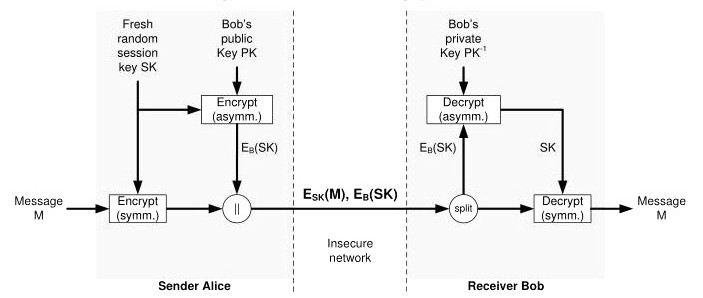
\includegraphics[width=12cm]{hybrid-encryption.jpg}
  \caption{Hybrid encryption.\label{abb_1}}
\end{figurehere}

\vspace{0.3cm} 

\noindent
The algorithm \textsc{eAES} is designed by Kovac and Underhill. They published the e-print \textit{Towards post-quantum symmetric cryptography} \cite{KUN} on the motivation for their research as well as the design and implementation of \textsc{eAES}. Underhill had previously started the implementation in his CEX-NET project, within which he created the cryptographic $C++$ library CEX \cite{CEX}. The library is open source and published under the GPL-license. Bogomolec is responsible for the mathematical analysis of the algorithm. All of us are independent IT-Security experts.\\

\noindent
\textsc{eAES} mitigates threats by formerly published attacks on \textsc{AES} from binary devices \cite{HFE,WEI,CRK} and additionally offers enhanced security against attacks performed by moderate quantum computers \cite{GRO,QAA}. \\ 

\section{Published attacks on \textsc{AES}}

\noindent
There are various types of attacks on cryptographic algorithms, amongst which side-channel attacks, implementation attacks, brute-force attacks and cryptanalysis attacks on \textsc{AES} are of importance in our context. In some cases, those attack types can be combined to achieve a more efficient decryption of a ciphertext.\\

\noindent
\textbf{Side-channel attacks} use unintended side effects of cryptographic operations to glean information about the plaintext and/or secret key being processed. \textbf{Implementation attacks} use weaknesses in implementation of an encryption scheme, e.g. weak key generation. \textbf{Brute force attacks} attempt every possible combination for a key. \textbf{Cryptanalysis attacks} rely on alternative algorithms for finding a secret key of an encrypted text. The latter can be applied to stationary data. Therefore it is interesting for data collectors who are patient enough to wait for the availability of potent enough machines to perform such an attack.

\subsection{Mathematical structure of \textsc{AES}}
\noindent
All basic \textsc{Rijndael} functions except \textit{SubBytes} are linear (see section Basic \textsc{Rijndael} encryption functions). The polynomial system which is represented by \textit{SubBytes} can be reduced to a Boolean equation system with the quantum algorithm  described in \cite{QAA}. Well chosen linear layers with very strong diffusion properties protect against conventional attacks using statistical properties of a cryptosystem. In the case of the quantum algebraic attack \cite{QAA}, this effect is limited.

\subsection{Attacks performed on binary devices}
\noindent
Various published attacks on \textsc{AES} \cite{HFE, WEI, CRK} take advantage of the invertibility of the original \textsc{Rijndael} key schedule besides other properties such as the relatively low number of rounds, implementation weaknesses and the same block size for standardized all key sizes.

\subsection{Grover's search}
\noindent
\textsc{AES} was generally still considered post-quantum secure for key sizes larger than $192$. Even Grover’s search algorithm \cite{GRV} is not regarded a threat for \textsc{AES}-$256$ in the near future. It can be used to extract the key from a small number of \textsc{AES} plaintext-ciphertext pairs ($5$ for \textsc{AES}-$256$). Grover's search is a alternative algorithm for an exhaustive key search (brute force attack).

\subsection{Quantum algebraic attack}
\noindent
A harder impact on the security of \textsc{AES}-$256$ is posed by the quantum algebraic attack on cryptosystems which can be reduced to Boolean equation solving \cite{QAA}. This attack reduces security level of \textsc{AES}-$256$ from $256$ to $78.53$, with a factor $\kappa^2$, the condition number of the Boolean equation system. The quantum algebraic attack is a classical cryptanalysis attack.

\subsection{Consequences}
\noindent
Both Grover's search algorithm and the quantum algebraic attack can be applied to collected data without the corresponding key exchanges as soon as potent enough quantum computers are available. Therefore we propose \textsc{eAES} as a symmetric alternative for \textsc{AES}, with higher security against all previously mentioned attacks \cite{HFE,WEI,CRK,GRO,QAA}.\\


% The command \subsection{Title} produces a subsection
\section{\textsc{Rijndael}, the base of \textsc{eAES}}

\noindent
Here we only give a high level overview of \textsc{Rijndael} in order to classify our modifications. For a detailed description of its standardized version \textsc{AES}, we refer to the Federal Information Processing Standards Publication $197$ \cite{AES}. 

\subsection{Computation grounds}
\noindent
\textsc{Rijndael} is an iterative rounds-based block cipher. It relies on a substitution-permutation network. In \textsc{AES}, the network is operating on a $4 \times 4$ column-major order array of the $128$ bits (block size), called the \glqq state\grqq. Each input data block is intially transformed into a \glqq state\grqq. The term \glqq state\grqq \, refers to the digital representation as well as to the fact of the continuous transformation during the encryption. So each array entry consists of $8$ bits. Columns of the matrix are also called \glqq words\grqq. All operations are performed in the Galois field $GF (2^8) \cong \mathbb{F}_2 [x]/(x^8 + x^4 + x^3 + x + 1 )$.


\subsection{\textsc{Rijndael} algorithm architecture}
\noindent
\textsc{Rijndael} is a block cipher. That means that the basic encryption functions are iterated a certain number of rounds with dedicated round keys over the state. With $r = $ number of rounds, the encryption process is:\\

\begin{itemize} [noitemsep, nolistsep]
\item[(1)] \textbf{Derive round keys}\\
Call \textit{ExpandKey}\,(key) to derive $r+1$ round keys from the secret key. The $+ 1$ stands for the fact that \textit{Add\-RoundKey} is called additionally before each block encryption. 
\vspace{0.1cm}
\item[(2)] \textbf{Encryption}\\
Perform on each block of data represented by the \glqq state\grqq: 
\vspace{0.1cm}
  \begin{itemize} [noitemsep, nolistsep]
    \item[a)] Initial round:
      \begin{itemize} [noitemsep, nolistsep]
        \item[] Add the plaintext to the state 
        \item[] \textit{AddRoundKey}\,(state, $1$st round key)
      \end{itemize} 
    \vspace{0.1cm}
    \item[b)] For ($i=2$; $i\leq r-1$, $i$++):
    \vspace{0.1cm}
    \begin{itemize} [noitemsep, nolistsep]
        \item[] \textit{SubBytes}\,(state) 
        \item[] \textit{ShiftRows}\,(state) 
        \item[] \textit{MixColumns}\,(state) 
        \item[] \textit{AddRoundKey}\,(state, $i$-th round key) 
    \end{itemize} 
    \vspace{0.1cm}
    ($4$ basic \textsc{Rijndael} encryption functions)
    \vspace{0.1cm}
    \item[c)] The final round:
    \begin{itemize} [noitemsep, nolistsep]
        \item[] \textit{SubBytes}\,(state)
        \item[] \textit{ShiftRows}\,(state)
        \item[] \textit{AddRoundKey}\,(state, last round key) 
    \end{itemize} 
  \end{itemize}
\end{itemize}
\vspace{0.5cm}

\noindent
The decryption process is composed by the inversed chain of the encryption functions. A symmetric encryption algorithm needs to be composed by invertible functions, but this property wouldn't be necessary for the key expansion. In fact, the invertibility of \textit{ExpandKey} opened the door for various side-channel attacks. 

\subsection{Basic \textsc{Rijndael} encryption functions}
The $4$ basic functions of the \textsc{Rijndael} encryption are: \\

\begin{itemize} [noitemsep, nolistsep]
  \item[1)] \textit{AddRoundKey} - addition in ${(\mathbb{F}_2)}^{128}$: \\ 
  Bitwise addition of the state and the correspondent round key.
  \vspace{0.1cm}

  \item[2)] \textit{SubBytes} - non-linear substitution: \\
  Each byte is replaced by another according to the specified substitution table ($S$-Box). A more resource friendly option is to treat a state byte as an element $\alpha \in \mathbb{F}_2 [x]/(x^8 + x^4 + x^3 + x + 1)$, where the multiplicative inverse of $\alpha$ needs to be found.
  \vspace{0.1cm}

  \item[3)] \textit{ShiftRows} - transposition for diffusion: \\
  The second, third and fourth row of the state are shifted to the left, by $1$, $2$ and $3$ steps.
  \vspace{0.1cm}

  \item[4)] \textit{MixColumns} - mixing for diffusion: \\
  Multiplication of each column of the state with the following matrix $M$:

  $$ 
  	M = 
  	\begin{bmatrix}
  		2 & 3 & 1 & 1 \\ 
  	 	1 & 2 & 3 & 1 \\
  	 	1 & 1 & 2 & 3 \\
  	 	3 & 1 & 1 & 2 \\
  	\end{bmatrix}
  $$

\end{itemize} 

\vspace{0.2cm}
\noindent
As a chain of invertible algebraic functions, \textsc{Rijndael} and \textsc{AES} can be represented as a polynomial system \cite{CCI}. This polynomial system can re reduced to a Boolean equation system. We will look at this property in the context of the quantum algebraic attack \cite{QAA}. \\

\section{Modifications for \textsc{eAES}}
\noindent
Our modifications affect the key schedule \textit{ExpandKey} and the number of rounds per version. Furthermore we implemented a version for a $512$-bit key, which is no outlier amongst post-quantum secure algorithm key sizes. \\

\subsection{\textsc{Rijndael} inheritance}
\noindent
The original \textsc{Rijndael} algorithm includes a block size option of $256$ bits, which was not admitted for the \textsc{AES} standard. We decided to keep the $128$ bits for \textsc{eAES} inorder to ensure compatibility with existing hardware implementations \footnote{We have also implemented an authenticated stream cipher (\textsc{RCS}) using the $256$-bit block transform along with a cryptographically strong key-schedule, and an increase in transformation rounds that parallels eAES.}. Several mentioned attacks take advantage of the fact that \textsc{AES}-$256$ runs with the same block size as \textsc{AES}-$128$. Those vulnerabilities are at least mitigated in our algorithm by the higher number of rounds. We also kept the $4$ basic \textsc{Rijndael} encryption functions and the \textsc{Rijndael} algorithm architecture.

\subsection{More rounds and a 512-bit key version}
\noindent
We increased the number of rounds taking in account recommendations of renowned cryptographers and cryptanalysts such as Bruce Schneier. The $256$-bit key variant \textsc{eAES}-$256$ runs $22$ rounds of the original \textsc{Rijndael} transformation function, which is $8$ more rounds than \textsc{AES}-$256$, and twice the best known attack which breaks $11$ rounds \cite{WEI}. Based on the same consi\-derations, we fixed the number of $30$ rounds for \textsc{eAES}-$512$ . 

\subsection{Say goodbye to 128- and 192-bit keys}
\noindent
Organizations such as the NIST and the EU quantum flagship \cite{KPN} recommend to use the maximal key lengths of currently used cryptographic algorithms whenever possible. But for operational staff in IT, the options very often simply come down to the question about what choices they have for establishing a confidential communication with a business or cooperation partner. \textsc{eAES} doesn't offer the $128$- and $192$-bit key options anymore.

\subsection{Replacing \textit{ExpandKey}}
\noindent
The invertibility of the original \textsc{Rijndael} key schedule \textit{ExpandKey} opened the door for various published attack schemes. Furthermore the output of the original \textsc{Rijndael} key schedule does not offer cryptographic quality. In the simple cases, round keys could be extracted within encryption or decryption processes, and the original key computed by applying the inverted key schedule function. For cryptanalysis attacks, this is just another convenient property for finding a replacement of the chain of \textsc{Rijndael} functions. \\
Therefore we replace \textit{ExpandKey} by cryptographically secure Pseudo Random Number Generators (PRNGs) with strong diffusion properties in \textsc{eAES}. 

\subsection{Pseudo Random Number Generators}
\noindent
PRNGs are built for deriving keys of a fixed size for further cryptographic operations by using an underlying pseudo random function. In our case those pseudo random functions are hashing algorithms. They are not even injective, but produce a well defined and collision resistant output. 

\begin{figurehere}
  \centering
  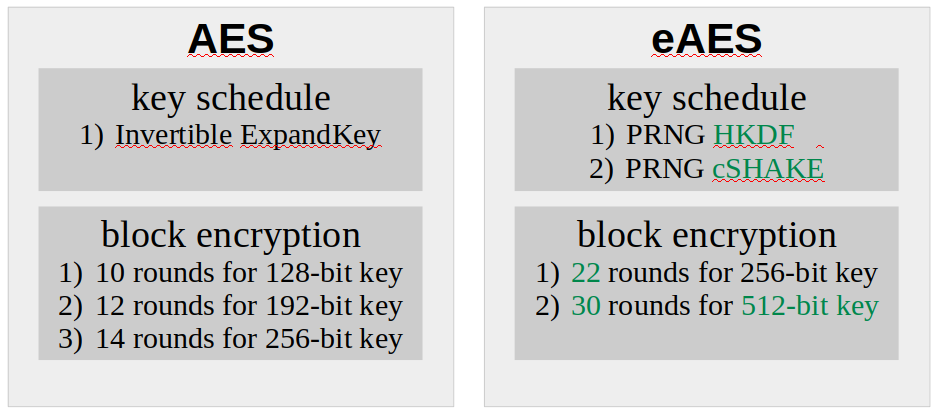
\includegraphics[width=10cm]{comparison.png}
  \caption{High level comparison of AES and eAES.\label{abb_2}}
\end{figurehere}
\vspace{0.3cm}

\noindent
Furthermore, it is very cost intensive under foreseeable technical developments to perform brute force attacks on the chosen PRNGs. So they are also hardly reversible apart from the non-existant mathematical invertibility.

\section{Key schedule variants}

\noindent
Our first choice is \textsc{HKDF}, a HMAC-based extract-and-expand key derivation function, with \textsc{SHA}-$2$ as the underlying hash function. As a second option, we implemented the \textsc{Keccak}-derived and customizable \textsc{cSHAKE}-function. \textsc{Keccak}, the \textsc{SHA}-$3$ competition finalist, was chosen by the NIST for its algorithmic unrelatedness from \textsc{SHA}-$2$, while offering flexibility and a comparable speed in computation. 

\subsection{Common features}
\noindent
Both \textsc{HKDF} and \textsc{cSHAKE} produce arrays of bytes which are converted to big-endian ordered $32$-bit integers for the round subkeys. Each round key has the same size as the cipher's block size, namely $128$ bits. So the output of our key derivation functions needs to be of the size $(r + 1)\cdot 128$ bit, where $r$ represents the number of rounds. We renounce on the usage of a salt due to the fact that within our algorithm, the input is cryptographically strong already.

\subsection{\textsc{HKDF}}
\noindent
We consider the \textsc{HMAC}-based \textsc{HKDF} as a sensible intermediary solution for the derivation of the round keys, because it is already widely available. We use \textsc{HKDF}(\textsc{SHA}-$256$) for \textsc{eAES}-$256$ and \textsc{HKDF}(\textsc{SHA}-$512$) for \textsc{eAES}-$512$ to align with expected security strengths. \\

\noindent
\textsc{SHA}-$256$ and \textsc{SHA}-$512$ are members of the \textsc{SHA}-$2$ function family. They use the Merkle-Damgard construction, a method of building collision-resistant cryptographic hash functions from collision-resistant one-way compression functions. The compression function for \textsc{SHA}-$2$ uses the Davies–Meyer structure from a (classified) specialized block cipher. \\ 

\noindent
\textsc{HKDF} generates cryptographically strong output of any desired length by repeatedly generating hash-blocks, concatenating them, and finally truncating the result to the desired length. 
Each call to \textsc{HMAC} involves two calls to the \textsc{SHA}-$2$ hash function to generate a pseudo-random $256$-bit or $512$-bit output block. \\

\noindent
So if the number of rounds is $r$ and the \textsc{SHA}-$2$ output length is $n$, \textsc{SHA}-$2$ has to be called $\lceil\frac{(r+1)\cdot128}{n}\rceil$ times. This results in $12$ times with \textsc{SHA}-$256$ for \textsc{eAES}-$256$ and $8$ times with \textsc{SHA}-$512$ for \textsc{eAES}-$512$.

\begin{figurehere}
  \centering
  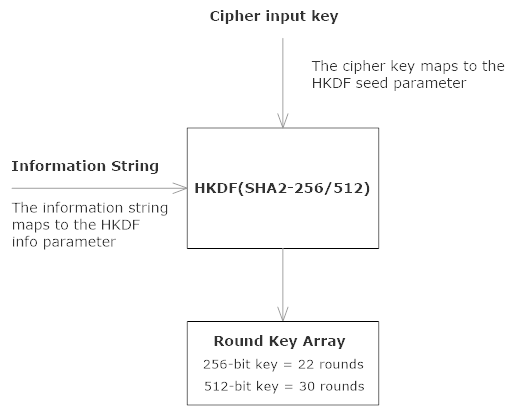
\includegraphics[width=8cm]{RHX-schematic.png}
  \caption{Rijndael HKDF eXtension.\label{abb_3}}
\end{figurehere}

\vspace{0.3cm}

\subsection{\textsc{cSHAKE}}

\noindent
We implemented the \textsc{SHA}-$3$-derived \textsc{SHAKE}-function as a second option for the key schedule. The \textsc{SHA}-$3$ competition finalist \textsc{Keccak} is a so called \textit{sponge function}. Those are functions with finite internal state, taking an input bit stream of any length and producing an output bit stream of any desired length. \textsc{cSHAKE} is the customizable version of \textsc{SHAKE}. It is originally designed for $128$- and $256$-bit security strength \cite{SHK}. Underhill has additionally created a $512$-bit security implementation, which mirrors the internal block-size, squeeze and permutation settings of \textsc{SHA3}-$512$. \textsc{cSHAKE}-$256$ is used for \textsc{eAES}-$256$, and \textsc{cSHAKE}-$512$ is used for \textsc{eAES}-$512$.\\

\noindent
The initial state of \textsc{SHAKE} is a $5 \times 5$ array of $64$-bit unsigned integers, $1600$ zero bits it total. The first call is to initialize the custom state. Then the original \textsc{eAES}-key is absorbed into the previously intialized state, and with each call to the inner permutation function of \textsc{Keccak}, rates of $(1600 - 2 \cdot n, \,\,  n \in \{ 256, 512 \})$ bits are returned. So \textsc{cSHAKE}-$256$ returns $136$, and \textsc{cSHAKE}-$512$ returns $72$ pseudo-random bytes per call.\\

\noindent
So if the number of \textsc{eAES}-rounds is $r$ and the number of returned bytes per rate are $n$, we have $\lceil\frac{(r+1) \cdot 128}{n \cdot 8}\rceil$ calls to the inner permutation functions of \textsc{cSHAKE}.For \textsc{eAES}-$256$ we have $3$ and for \textsc{eAES}-$512$ we have $7$ calls to the inner permutation function, $+ 1$ call for the initial state.\\

\begin{figurehere}
  \centering
  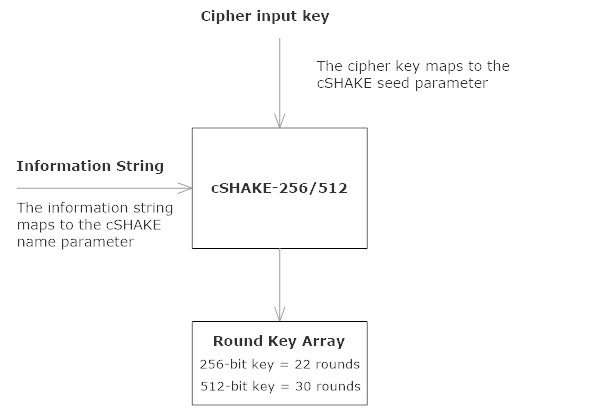
\includegraphics[width=8cm]{RSX-schematic.png}
  \caption{Rijndael SHAKE eXtension.\label{abb_4}}
\end{figurehere}

\vspace{0.3cm}

\noindent
Note that here we are talking about calls to the inner permutation function of \textsc{Keccak}, while we are talking about calls to \textsc{SHA}-$2$ itself in the previous section. Fewer calls of the permutation function lead to higher efficiency of \textsc{cSHAKE} compared to the one of \textsc{HKDF}. On the other hand, \textsc{Keccak} is prone to quantum algebraic attacks \cite{QAA}.

\section{Impact of Grover's Search Algorithm}

\noindent
Grover’s algorithm offers a $\sqrt{k}$ speed-up \cite{GRV} over a classical exhaustive search (brute force attack) on the set of keys of size $k$. It seems to be one of the most relevant quantum cryptanalytic impact for the study of block ciphers. The authors of \cite{GRO} present quantum circuits to implement the key search for \textsc{AES} and analyze the quantum resources required to carry out such an attack for key sizes of $128$, $192$ and $256$ bits. \\

\noindent
The number of required logical qubits is relatively low, $6,681$ for \textsc{AES}-$256$. On the other hand, the large circuit depth of enrolling the entire Grover iteration poses a challenge to an implementation on an actual physical quantum computer, even if the gates (basic quantum circuit operating on qubits) are not error corrected. The key schedule \textit{ExpandKey} causes much of the circuit cost within each Grover iteration. Replacing it by our chosen PRNGs will even be considerably more cost intensive. \\

\noindent
Here we only summarize the basic prerequisites of the involved procedures described in \cite{GRO} for \textsc{AES}-$256$ and compare them to \textsc{eAES} for $k \in \{256, 512\}$.

\subsection{Algorithm architecture}
\noindent
A quantum circuit implementing a Boolean function $f$ is the input of the Grover's search algorithm:
$$f: \{ 0,1 \}^k \rightarrow \{ 0,1 \} $$

\noindent
The basic algorithm finds an element $x_0$ such that $f(x_0)=1$. This is realized by repeatedly applying the operation $G$ to measure an element $x_0$ such that $f(x_0)=1$ with constant probability.
$$ G =U_f \left((H^{\otimes k} (2 |0\rangle \langle 0| -1_{2^k})H^{\otimes k})\otimes 1_2 \right)$$
$H$ denotes the $2 \times 2$ Hadamard transform and $U_f$ involves the computation of the cipher functions. To ensure uniqueness of the solution (the found key), a small number of plaintext-ciphertext pairs are needed. This number is $5$ for a $256$-bit key and $9$ for $512$-bit key.

\subsection{Quantum resources and graph theory}
\noindent
Quantum resources are represented by logical qubits, gates and circuit depth. In the model of a Boolean circuit as a directed acyclic graph, the circuit depth is the maximal length of a path from an input gate to the output gate. The sum of required gates represent the complexity of an algorithm.\\

\noindent
Reversible circuits are needed for the application of Grover on \textsc{AES} to provide invertibilty of the operations. Therefore the proposed solution in \cite{GRO} relies on a set of fault-tolerant reversible logical gates. It consists of called Toffoli gates, controlled NOT gates and NOT gates. A Toffoli gate is a universal reversible logic gate, i.e. any reversible circuit can be constructed from Toffoli gates. \\

\begin{figurehere}
  \centering
  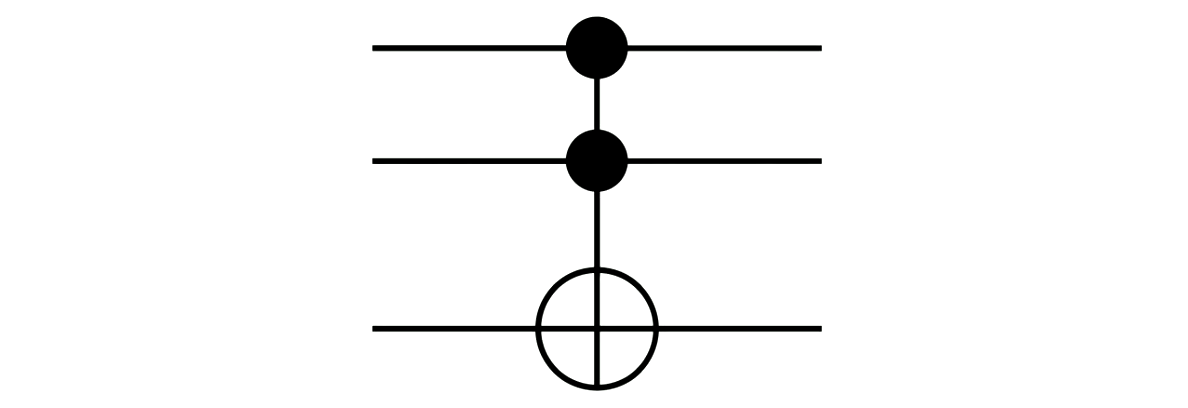
\includegraphics[width=12cm]{Toffoli.png}
  \caption{Toffoli gate (controlled-controlled-not gate).\label{abb_5}}
\end{figurehere}
\vspace{0.3cm}

\noindent
For our key schedule replacements, we will base our comparisons on the results of \glqq Estimating the cost of eneric quantum pre-image attacks on SHA-2 and SHA-3s\grqq \, \cite{QSH}. The authors present an implementation including Grover's algorithm on reversible circuits on on a surface code based fault-tolerant quantum computer.

\subsection{Quantum resources for the search}
\noindent
$H$ represents the Hadamard operation on a single qubit. A single solution to the equality function $f$ can be found by applying $H^{\otimes k+1}$ to the initial state, where $k$ is the size of the key. The next step is applying 
$$G^{\lceil \frac{\pi}{4} \sqrt{2^k}\rceil},$$ 
followed by a measurement of the entire quantum register which will yield a solution $x_0$ with high probability.\\

\noindent
The exact decomposition of the search is outlined in \cite{GRO}, section $2$. For our comparison we only look at the cost for the operation $(2 |0\rangle \langle 0| -1_{2^k}))$, which is determined by the reduction to the implementation of a $k$-fold NOT gate, where $k \in \{256,512\}$ is the key size. In terms of Toffoli gates we have the formula $8k-24$ \cite{EQC} and if we count only T-gates, we have the formula $32k-84$ as an upper bound for a $k$-fold controlled NOT gate \cite{QAN}. This results in:

  \begin{center}
  \textbf{Table 1: Cost for the operation $(2 |0\rangle \langle 0| -1_{2^k}))$}: \\
  \vspace{0.2cm}
    \begin{tabular}{c|c|c}
    key size & Toffoli gates & T-gates \\
    \hline
      &  &  \\ [-8pt]
    256               &    2,024                &  8,108    \\ 
    512               &    4,072                &  16,300     \\  
    \end{tabular}
  \end{center}
  \vspace{0.5cm}

\noindent
Grover's search will have to be performed on the small number $n$ of plaintext-ciphertext pairs. The equality function $f$ can be implemented by a multiple controlled NOT gate that has $128\cdot n$ controls. With above formulas, the needed number of Toffoli counts and T-counts to compute the equality function $f$ come down to: 

\begin{center}
\textbf{Table 2: ost for the equality function $f$:} \\
  \vspace{0.2cm}
  \begin{tabular}{c|c|c}
  key size & Toffoli counts & T-counts \\ 
  \hline
    &  &  \\ [-8pt]
  256               &    5,096                &  20,396    \\
  512               &    9,192                &  36,780     \\  
  \end{tabular} 
\end{center}
\vspace{0.5cm}

\noindent
The search resources only depend on the key sizes and not on the ciphers and their options. In this regard we don't have to include further differing considerations.

\subsection{Quantum resources for the ciphers}
\noindent
The number of rounds depends on the specific key length $k$, while the four basic \textsc{Rijndael} functions are independent of the key length $k$ for both \textsc{AES} and \textsc{eAES}. The realization of all \textsc{Rijndael} functions is analyzed in dedicated sections in \cite{GRO}. Here we only present the results and comparisons per function.\\


\begin{center}
\textbf{Table 3: Cost for SHA-2 and -3 functions (256 bit):} \\
\vspace{0.2cm}
  \begin{tabular}{l|c|c|c}
  function &  gates & depth & qubits \\ 
  \hline
    &  &  & \\ [-8pt]
  \textsc{SHA}-$256$ & $1.42 \cdot 2^{146}$ & $1.69 \cdot 2^{144}$ & $2^{12.6}$  \\  
  \textsc{SHA3}-$256$ & $1.52 \cdot 2^{147}$ & $1.33 \cdot 2^{137}$ & $2^{20}$  \\ 
  \end{tabular} 
\end{center}
\vspace{0.5cm}

\noindent
The values for \textsc{SHA}-$256$ and \textsc{SHA3}-$256$ are results from the resource estimates done in \cite{QSH}, converted to a representation in powers of $2$ instead of $10$. For both functions, the total cost comes down to approximately $2^{166}$ basic operations. The estimation of the resources for the according $512$-bit versions will be done in a further step of our research. \\

\noindent
For our \textsc{eAES}-options we have to multiply the gate values by the number of calls to the hash and inner permutation functions.

\begin{center}
\textbf{Table 4: Cost for \textsc{AES} and \textsc{eAES} key expansion (256 bit):} \\
\vspace{0.2cm}
  \begin{tabular}{l|c|c|c}
  function &  gates & depth & qubits \\ 
  \hline
    &  &  & \\ [-8pt]
  \textit{ExpandKey} & 54,331  &  23,896 & 512 \\
  \textsc{HKDF} & $1.07 \cdot 2^{150}$ & $1.26 \cdot 2^{148}$ & $2^{12.6} + 3072$  \\  
  \textsc{cSHAKE} & $1.52 \cdot 2^{149}$ & $1.33 \cdot 2^{139}$ & $2^{20} + 1024$  \\  
  \end{tabular} 
\end{center} 
\vspace{0.5cm}

\noindent
The numbers of gates and depths take the number of calls to the according hash and permutation functions into account. Additional qubits are needed to store the output of all calls to the hash functions.\\

\noindent
As mention before, we cannot refer to values for $512$-bit keys at this time. But we can see that the $256$-bit versions already offer considerable advantages over the original \textsc{Rijndael} key schedule \textit{ExpandKey}. \\

\begin{center}
\textbf{Table 5: Cost for holding the state and initial round:} \\
\vspace{0.2cm}
  \begin{tabular}{l|c|c|c}
  function &  gates & depth & qubits \\ 
  \hline
    &  &  & \\ [-8pt]
  state & 0  &  0 & 128 \\
  initial round $v_1$ & 64 NOT & 0 & 128  \\ 
  initial round $v_2$ & 128 CNOT & 1 & 256  \\ 
  \end{tabular} 
\end{center}
\vspace{0.5cm}

\noindent
Initial round $v_1$ represents the realization with flipping bits. These values are the same for all ciphers and options. \\

\begin{center}
\textbf{Table 6: Cost for basic functions} \\
\vspace{0.2cm}
  \begin{tabular}{l|c|c|c}
  function &  gates & depth & qubits \\ 
  \hline
    &  &  & \\ [-8pt]
  \textit{SubBytes} & 22,326  &  1 & 9 \\
  \textit{ShiftRows} & 0 & 0 & 0  \\ 
  \textit{MixColumns} & 277 CNOT & 39 & 0 \\
  \textit{AddRoundKey} & 128 CNOT &  1 & 0 \\ 
  \end{tabular} 
\end{center}
\vspace{0.5cm}

\noindent
The current round key is available on $128$ dedicated wires. \textit{SubBytes} is realized by finding the inverse of the byte in $GF (2^8)$, seen as permutation in $\mathbb{F}_{256}$.  No extra gates are necessary to implement \textit{ShiftRows}, as it corresponds to a permutation of the qubits. The position of the subsequent gates is simply adjusted to the correct input wire. \\

\begin{center}
\textbf{Cost for \textsc{Rijndael} rounds} \\
\end{center}

\noindent
To compute all rounds of \textsc{Rijndael}, $536$ qubits are needed for $10$ rounds in the $128$ bit key version and $664$ qubits are required for any round number $r \geq 12$. In this regard, the higher number of rounds in \textsc{eAES} does not add complexity to the algorithm. But the number of rounds do add complexity to the number of gates and to the depth. \\

\begin{center}
\textbf{Cipher output for 256 bit keys} \\
\end{center}

\noindent
The number of gates and depth for \textsc{eAES} is derived as follows: \\

\noindent
Values from the rounds row in table $4$, \textsc{AES}-$256$ in \cite{GRO} : \\ 

\noindent
$g_{14}=$ sum of number of gates in \cite{GRO} \\
$d_{14}=$ sum of depths in \cite{GRO} \\

\noindent
Values from the key expansion cost table in this article: \\

\noindent
$g_{hkdf}=$  number of gates for \textsc{HKDF}-$256$ \\
$d_{hkdf}=$  depths for \textsc{HKDF}-$256$ \\
$q_{hkdf}=$  number of qubits for \textsc{HKDF}-$256$ \\
$g_{shake}=$ number of gates for \textsc{cSHAKE}-$256$ \\
$d_{shake}=$ depths for \textsc{cSHAKE}-$256$ \\
$q_{shake}=$ number of qubits for \textsc{cSHAKE}-$256$ \\

\noindent
Then we compute the values for \textsc{eAES}(\textsc{HKDF}) from the formulas:\\
\vspace{0.5cm}
\noindent
$\small{gates} = g_{hkdf} + \frac{22}{14} \cdot g_{14} \,\,$
$\small{depth} = d_{hkdf} + \frac{22}{14} \cdot d_{14}$

\noindent
The values for \textsc{eAES}(\textsc{cSHAKE}) from the formulas: \\
\vspace{0.5cm}
\noindent
$\small{gates} = g_{shake} + \frac{22}{14} \cdot g_{14}, \,\,$
$\small{depth} = d_{shake} + \frac{22}{14} \cdot d_{14}$

\noindent
And the number of qubits for is the simple addition $664 + q_{sha}$ , $664 + q_{sha3}$ respectively. \\

\begin{center}
\textbf{Table 7: Cost for each cipher output (256 bit)} \\
\vspace{0.2cm}
  \begin{tabular}{l|c|c|c}
  cipher &  gates & depth & qubits \\ 
  \hline
    &  &  & \\ [-8pt]
  \textsc{AES}-256 & $1.65 \cdot 2^{21}$  &  $1.46 \cdot 2^{17}$ & 1,336 \\
  \small{\textsc{eAES}(\tiny{\textsc{HKDF}})} & $1.07 \cdot 2^{150}$ & $1.26 \cdot 2^{148}$ & $1.21 \cdot 2^{13}$  \\  
  \small{\textsc{eAES}(\tiny{\textsc{cSHAKE}})} & $1.52 \cdot 2^{149}$ & $1.33 \cdot 2^{139}$ & $1.002 \cdot 2^{20}$  \\  
  \end{tabular} 
\end{center}

\noindent
Note that the gates and depth values for \textsc{eAES} equal the values in the key expansion cost table. This comes from the fact that the contribution of the gates and and depth from the rounds is in much lower power of $2$ than the cost for the key expansions \textsc{HKDF} and \textsc{cSHAKE}. So we see that this replacements are the essential change and contribution to a higher algorithm complexity. \\

\begin{center}
\textbf{Grover algorithm} \\
\end{center}

\noindent
For the overall T-count for Grover on \textsc{Rijndael} we have an estimate of $\lfloor \frac{\pi}{4} 2^{k/2}\rfloor \cdot (6 t_{k} + f_k)$, where $k$ is the key size, $t_k$ is the number of T-gates and $f_k$ is the cost for the equality function. For the overall circuit depth we obtain with $r=$ number of rounds: $2 \cdot r \cdot$ total T-depth. Here we are ignoring some of the gates which do not contribute significantly to the bottom line. Both formulas are from \cite{GRO}, section 3.4.. So by a moderate estimation we get the following complexities for Grover's search on the compared ciphers:\\ 

\begin{center}
\textbf{Table 8: Grover's search on ciphers} \\
\vspace{0.2cm}
  \begin{tabular}{l|c|c|c}
  cipher &  gates & depth & qubits \\ 
  \hline
    &  &  & \\ [-8pt]
  \textsc{AES}-$256$ & $3.24 \cdot 2^{151}$  & $1.71 \cdot 2^{145}$  & 6,681 \\
  \small{\textsc{eAES}(\tiny{\textsc{HKDF}})} & $> 2^{278}$ & $ > 2^{274}$ & $>  2^{14}$  \\  
  \small{\textsc{eAES}(\tiny{\textsc{cSHAKE}})} & $> 2^{277}$ & $ > 2^{257}$ & $> 2^{21}$  \\  
  \end{tabular} 
\end{center}
\vspace{0.5cm} 

\noindent
Both \textsc{HKDF} and \textsc{cSHAKE} have a considerable impact on the increased cost of Grover's search. The higher number of rounds for \textsc{eAES}-$256$ and the $512$-bit key version additionally contibute to the complexity of the rounds by factors of at least $\frac{r}{14}$. The authors of \cite{GRO} recommended in $2015$ to move away from \textsc{AES}-$128$ when expecting the availability of at least a moderate size quantum computer. Our implementation excludes that option and offers an increased complexity of at least $2^{126}$ compared to \textsc{AES}-$256$. \\

\section{Impact of Quantum Algebraic Attacks}

\noindent
The authors of \cite{QAA} present an algorithm which leads to new considerations of the security of systems which can be reduced to solving Boolean equations. A solution $a$ for the equation $\mathcal{F} \cdot a = 0$ with a set of polynomials $\mathcal{F} \subset \mathbb{C}[X]$ is called \textit{Boolean} if each coordinate of $a$ is either $0$ or $1$.\\

\noindent
The resulting quantum algebraic attack algorithm includes quantum-monomial solving of polynomial systems over $\mathbb{C}$ by applying a Macaulay linear system. The authors construct a Boolean equation solving algorithm, with the following properties: \\

\begin{itemize} [noitemsep, nolistsep]
  \item[1)] It decides if there exists a Boolean solution.
  \vspace{0.1cm}
  \item[2)] It returns a Boolean solution with a given probability if there are such solutions to the system.
  \vspace{0.1cm}
  \item[3)] It returns $\emptyset$ if no Boolean solution exists.
\end{itemize}
\vspace{0.5cm}

\noindent
The conclusion of \cite{QAA} is, that systems which can be solved by Boolean equation solving, are only secure under quantum algebraic attack, if the condition number $\kappa$ is large. The construction of such systems is a topic for further research. Besides \textsc{AES} and \textsc{Keccak}, stream ciphers such as \textsc{Trivium} an the multivariate public key cryptosystem \textsc{MPKC} are affected by the attack. \\

\noindent
The runtime complexity of the resulting quantum algebraic attack is considerably lower than the one of Grover's Search, but it depends on two factors: the complexity constant $c$ of the underlying \textsc{HHL} quantum algorithm \cite{HHL} and the condition number $\kappa$ of their specified Macaulay matrix from the involved polynomial system. The complexity of $2^{78.53}c\kappa^2$ for \text{AES}-$256$ is not much higher than the complexity of $2^{73.30}c\kappa^2$ for \text{AES}-$128$ due to the same block size of $128$ bit. \\

We can assume that the complexity won't be much higher for $512$-bit key sizes, and it will also not considerably increased by the higher number of rounds in \textsc{eAES}. In the case of \textsc{eAES} it has to be investigated if dedicated polynomial systems can be derived for the usage of either key schedule options, \textsc{HKDF} and \textsc{cSHAKE}. Both huge Macaulay matrices need to be generated explicitly to actually compute $\kappa_{AES}$ and $\kappa_{Keccak}$ to derive the complexity of the Quantum Algebraic Attack on eAES. The ongoing research project team regularly publishes results on Github \cite{XBO}.\\

%check impact of rounds and key schedules!!!


\section{Conclusion}

\noindent
Considering the lower exponent of the highest power of $2$ in the total algorithm complexity, \textsc{eAES} offers a higher complexity of a factor $\geq 2^{277-151}=2^{126}$ regarding Grover's search algorithm compared to  \textsc{AES}, even if only the $256$-bit version is used. Regarding the quantum algebraic attacks, it remains to be investigated if there are Boolean multivariate quadratic equations for both key schedule versions, \textsc{HKDF} and \textsc{cSHAKE}.\\

\noindent
We consider \textsc{eAES} a sensible candidate for a first generation post-quantum secure symmetric encryption. It runs effectively on currently used devices and is compatible with existing hardware implementations. We hope to be able to contribute to a smooth transition into the new post-quantum cryptographical era.


\vspace{2cm}

%%% For figures
%\begin{figurehere}
%  \centering
%  \includegraphics[width=12cm]{Abbildung}
%  \caption{First figure of this article.\label{abb_1}}
%\end{figurehere}

%%%%%%%%%%%%%%%%%%%%%%%%%%%%%%%%%%%%%%%%%%%%%%%%%%%%%%%%%%%%%%%%%%%%%%%%%%%%%%%%
% Literature
%%%%%%%%%%%%%%%%%%%%%%%%%%%%%%%%%%%%%%%%%%%%%%%%%%%%%%%%%%%%%%%%%%%%%%%%%%%%%%%%

\begin{thebibliography}{1}
\itemsep=0cm plus 0pt minus 0pt

\bibitem{MSN}
  S.~Shankland,
  \newblock MSN News,
  \newblock { \em https://www.msn.com/en-us/news/technology/ibms-new-53-qubit-quantum-computer-is-its-biggest-yet/ar-AAHtPaW}, September 2019.

\bibitem{googleai}
  J.~Kelly,
  \newblock Google AI Blog,
  \newblock {https://ai.googleblog.com/2018/03/a-preview-of-bristlecone-googles-new.html}, March 2018.

\bibitem{TQB}
  S.~Ran, C.~Eckberg, Q.-P.~Ding, Y.~Furukawa, T.~Metz, S.R.~Saha, I-L.~Liu, M.~Zic, H.~Kim, J.~Paglione and N.P.~Butch,
  \newblock NIST events on paper of above authors,
  \newblock { \em https://www.nist.gov/news-events/news/2019/08/newfound-superconductor-material-could-be-silicon-quantum-computers}.

\bibitem{KUN}
S.~Kovac and J.~Underhill,
\newblock Towards post-quantum symmetric cryptography,
\newblock {\em https://eprint.iacr.org/2019/553}.

\bibitem{CEX}
J.~Underhill,
\newblock The CEX Cryptographic library in C++,
\newblock {\em https://github.com/Steppenwolfe65/CEX}.

\bibitem{HFE}
A.~Biryukov and D.~Khovratovich,
\newblock Related-key Cryptanalysis of the Full AES-192 and AES-256,
\newblock {\em https://eprint.iacr.org/2009/317.pdf}.

\bibitem{WEI}
A.~Biryukov, O.~Dunkelman, N.~Keller, D.~Khovratovich and A.~Shamir
\newblock Key Recovery Attacks of Practical Complexityon AES-256 Variants With Up To 10 Rounds
\newblock {\em http://www.wisdom.weizmann.ac.il/~orrd/crypt/PracticalAES256.pdf}.

\bibitem{CRK}
S.~Lucks,
\newblock Attacking Seven Rounds of \textsc{Rijndael} under 192-bit an 256-bit Keys,
\newblock {\em https://madoc.bib.uni-mannheim.de/10615/}, 2000.

\bibitem{GRO}
M.~ Grassl, B.~ Langenberg, M.~ Roetteler, R.~ Steinwandt,
\newblock Applying Grover’s algorithm to AES: quantum resource estimates,
\newblock {\em https://arxiv.org/abs/1712.06239}, 2018.

\bibitem{QAA}
Y.~-A.~Chen, X.~-S.~Gao,
\newblock Quantum Algorithms for Boolean Equation Solving and Quantum Algebraic Attack on Cryptosystems,
\newblock {\em https://arxiv.org/abs/1712.06239}, 2018.

\bibitem{HHL}
A.W. Harrow, A.Hassidim, S.Lloyd, 
  \newblock Quantum algorithm for linear systems equations, 
  \newblock  { \em Physical Review Letters, 103(15)}: 150502, 2009. 

\bibitem{GRV}
L.~K.~Grover,
\newblock A fast quantum mechanical algorithm for database search, 
\newblock { \em Gary L. Miller, editor, Proceedings of the
Twenty-Eighth Annual ACM Symposium on the Theory of Computing (STOC 1996), pages 212–219} ACM, 1996.

\bibitem{AES}
Federal Information Processing Standards Publication 197, NIST,
\newblock Announcing the ADVANCED ENCRYPTION STANDARD (AES),
\newblock {\em https://csrc.nist.gov/csrc/media/publications/fips/\-197/final/documents/fips-197.pdf}, 2000.

\bibitem{CCI}
C.~Cid, Information Security Group, University of London,
\newblock Algebraic Analysis of AES,
\newblock {\em https://www.cosic.esat.kuleuven.be/ecrypt/AESday/\-slides/AES-Day-CarlosCid.pdf}, October 2012.

\bibitem{KPN}
J.~Baloo, KPN,
\newblock Everything is Quantum – The EU Quantum Flagship, 
\newblock { \em https://2017.pqcrypto.org/conference/slides/baloo.pdf}, 2017.

\bibitem{SHK}
J.~Kelsey, S.~-J.~Chang, ~R.~Perlner,
\newblock SHA-3 Derived Functions: cSHAKE, KMAC, TupleHash and ParallelHash, 
\newblock { \em https://nvlpubs.nist.gov/nistpubs/SpecialPublications
/NIST.SP.800-185.pdf}, December 2016.

\bibitem{QSH}
M.~Amy, O.~Di Matteo, V.~Gheorghiu, M.~Mosca, A.~Parent, J.~Schanck,
\newblock Estimating the cost of eneric quantum pre-image attacks on SHA-2 and SHA-3s, 
\newblock { \em https://eprint.iacr.org/2016/992.pdf} QCrypt, 2016.

\bibitem{EQC}
A.~Barenco, C.~H.~Bennett, R.~Cleve, D.~P.~DiVincenzo, N.~Margolus, P.~W.~Shor, T.~Sleator, J.~Smolin, H.~Weinfurter,
\newblock Elementary gates for quantum computation, 
\newblock { \em Physical Review A, 52(5):3457–3467}, 1995.

\bibitem{QAN}
N.~Wiebe and M.~Roetteler,
\newblock Quantum arithmetic and numerical analysis using Repeat-Until-Success circuits, 
\newblock { \em https://arxiv.org/abs/1406.2040}, 2014.

\bibitem{XBO}
P.~Nonnenmann and X.~Bogomolec,
\newblock Complexity of the Quantum Algebraic Attack on AES:
The Condition Number of the Macaulay Matrix, 
\newblock { \em https://github.com/XeniaGabriela/QAA\_Condition\_Nr/blob/master/official\_paper/QAA\_on\_AES\_paper.pdf}, 2020.
  
\end{thebibliography}

%%%%%%%%%%%%%%%%%%%%%%%%%%%%%%%%%%%%%%%%%%%%%%%%%%%%%%%%%%%%%%%%%%%%%%%%%%%%%%%%


%%% IF ENGLISH:
\end{otherlanguage}
%%%

\end{document}
